\documentclass[a4paper,14pt]{article}

\usepackage{fvextra}
\usepackage{verbatim}

\DefineVerbatimEnvironment{Verbatim}{Verbatim}{breaklines=true}



\usepackage{eso-pic}


\usepackage{float}
\usepackage{graphicx}

\usepackage{listings}
\usepackage{xcolor}

\usepackage[utf8]{inputenc}
\usepackage[english, russian]{babel}


\setlength{\parindent}{12.5mm} 



\lstset{
    basicstyle=\ttfamily\small, % Шрифт и размер
    breaklines=true,             % Перенос строк
    breakatwhitespace=false,     % Перенос по пробелам
    columns=flexible,            % Гибкий размер колонок
%     frame=single,                % Рамка вокруг кода
%     backgroundcolor=\color{lightgray!20}, % Цвет фона
}


\usepackage{calc}
\usepackage{background}


\usepackage[height=297mm, width=210mm, left=3cm, top=2cm, right=1cm, bottom=2cm]{geometry}


\newcommand{\chipher}{
        {\fontsize{16pt}{16pt}\selectfont  КР.ИИ-21.210574-3 81 00}
}


\begin{document}
        \sloppy
        
        \pagestyle{empty}
        \fontsize{14}{17.5}\selectfont    


        


\newcommand{\applicationTitlePage}{

    \begin{center}
        МИНИСТЕРСТВО ОБРАЗОВАНИЯ РЕСПУБЛИКИ БЕЛАРУСЬ \\
        УЧРЕЖДЕНИЕ ОБРАЗОВАНИЯ \\
        <<БРЕСТСКИЙ ГОСУДАРСТВЕННЫЙ ТЕХНИЧЕСКИЙ УНИВЕРСИТЕТ>> \\
        ФАКУЛЬТЕТ ЭЛЕКТРОННО-ИНФОРМАЦИОННЫХ СИСТЕМ \\
        Кафедра интеллектуальных информационных технологий \\[4cm]
        
         
            \MakeUppercase{
                {\bf Приложение А \\}
                
            }
            <<Текст программы>> \\[4cm]
        
           
            
        

    \end{center}

    \begin{flushright}
        \begin{minipage}{0.35\textwidth}
            \begin{flushleft}
                {\bf Выполнил:} \\
                студент 4-го курса, \\
                ФЭИС, \\
                группы ИИ-21 \\
                Литвинюк Т. В. \\
                {\bf Проверил:} \\
                Кулеша В. И.
            \end{flushleft}
        \end{minipage}
    \end{flushright}

    \vfill 

    \begin{center}
        Брест \the\year
    \end{center}

    \newpage

}



        \newcommand{\content}{
    % добавляем нумерацию
    \AddToShipoutPicture{
        \begin{textblock*}{1cm}(19.5cm,28.6cm) % Ширина блока, координаты (x, y)
                \centering 
                \number\numexpr\thepage+1\relax
        \end{textblock*}
    }

    % добавляем шифр
    \AddToShipoutPicture{
        \begin{textblock*}{10cm}(9cm,28.2cm) % Ширина блока, координаты (x, y)
            \centering
            \chipher
        \end{textblock*}
    }

    % шифр на 1ый лист
    \begin{textblock*}{10cm}(9cm,28.2cm) % Ширина блока, координаты (x, y)
        \centering
        \chipher
    \end{textblock*}

    

\section*{\MakeUppercase{Введение}}
\addcontentsline{toc}{section}{Введение}
    {
        В современном мире стремительное развитие технологий оказывает значительное влияние на различные аспекты жизни, включая кулинарию. С появлением искусственного интеллекта (ИИ) и нейронных сетей стали доступны новые подходы к решению задач, связанных с обработкой больших объемов данных, персонализацией опыта пользователей и автоматизацией рутинных процессов. Одним из таких подходов является использование ИИ для поиска и подбора кулинарных рецептов, что делает процесс готовки более удобным и увлекательным.
        
        Целью данного курсового проекта является разработка веб-приложения, которое предоставляет пользователям возможность находить рецепты блюд на основе заданных ингредиентов с использованием нейронной сети. Особенностью приложения является способность оптимизировать поиск: если заданный запрос уже встречался ранее, данные извлекаются из базы данных, что ускоряет отклик системы. Если запрос уникален, приложение отправляет запрос к языковой модели (нейронной сети, представленной сервером ChatGPT-4o) для генерации списка рецептов. Кроме того, реализована возможность авторизации пользователей и сохранения истории запросов, что делает систему персонализированной.
        
        Данное веб-приложение призвано решить следующие задачи:
        \begin{enumerate}
            \item Упростить поиск рецептов, используя интуитивно понятный интерфейс.
            \item Минимизировать задержки за счет кэширования результатов запросов.
            \item Обеспечить удобное хранение истории запросов для каждого пользователя.
            \item Демонстрировать потенциал интеграции технологий ИИ в веб-приложения.
        \end{enumerate}

        В результате разработки данного приложения пользователи смогут быстро находить рецепты, улучшая свои кулинарные навыки, а также познакомятся с практическим использованием современных технологий искусственного интеллекта в повседневной жизни. 
        
        Работа структурирована следующим образом: в первой части описывается постановка задачи и обоснование выбора технологий, во второй — разработка веб-приложения, включая создание интерфейса, баз данных и интеграции с ИИ, а в заключении — анализ полученных результатов и выводы.
    }
    \newpage

\newpage

\section{\MakeUppercase{Постановка задачи}}


\subsection*{Цель работы}
Целью данного курсового проекта является разработка веб-приложения для поиска кулинарных рецептов, которое использует нейронную сеть для генерации уникальных рецептов на основе введенных пользователем ингредиентов. Приложение также должно оптимизировать обработку запросов, используя базу данных для хранения и извлечения ранее запрашиваемых данных.

\subsection*{Основные задачи}
Для достижения цели необходимо решить следующие задачи:
\begin{enumerate}
    \item Разработать пользовательский интерфейс, позволяющий вводить список ингредиентов и получать рецепты.
    \item Реализовать авторизацию и регистрацию пользователей, чтобы предоставлять персонализированный опыт и сохранять историю запросов.
    \item Создать базу данных для хранения рецептов и истории запросов пользователей с использованием PostgreSQL.
    \item Интегрировать приложение с языковой моделью (ChatGPT-4o) для генерации рецептов, если запрашиваемые ингредиенты отсутствуют в базе данных.
    \item Разработать механизм кэширования запросов, чтобы ускорить обработку повторяющихся запросов.
    \item Обеспечить защиту данных пользователей, соблюдая принципы безопасной разработки.
\end{enumerate}

\subsection*{Ожидаемые результаты}
В результате выполнения проекта должно быть разработано веб-приложение, которое:
\begin{itemize}
    \item позволяет пользователям вводить ингредиенты для поиска рецептов;
    \item возвращает рецепты, извлекая их либо из базы данных, либо из ответа нейронной сети;
    \item сохраняет запросы пользователей, обеспечивая удобный доступ к истории;
    \item демонстрирует эффективность использования искусственного интеллекта для решения практических задач.
\end{itemize}

Данное приложение должно быть интуитивно понятным и удобным в использовании, а также демонстрировать основные преимущества интеграции нейронных сетей в веб-разработку.

\newpage
  
\section{\MakeUppercase{Выбор и описание используемых инструментов}}
{
    \subsection{Модель машинного обучения}
    В рамках данного проекта для генерации кулинарных рецептов на основе введённых ингредиентов была выбрана языковая модель ChatGPT-4o, предоставляемая OpenAI. Данная модель основана на архитектуре трансформеров и представляет собой мощный инструмент для обработки естественного языка. Её применение позволяет эффективно решать задачи генерации текстов, в том числе создание уникальных рецептов.

\subsubsection*{Обоснование выбора модели}
Выбор модели ChatGPT-4o обусловлен следующими преимуществами:
\begin{itemize}
    \item \textbf{высокая точность генерации текста.} Модель обучена на обширных наборах данных, что позволяет ей создавать тексты, соответствующие заданным требованиям;
    \item \textbf{гибкость.} Модель может адаптироваться под различные задачи, включая генерацию рецептов, обработку запросов и предоставление релевантных ответов;
    \item \textbf{интеграция через API.} ChatGPT-4o легко интегрируется в веб-приложения с использованием API, что упрощает процесс разработки;
    \item \textbf{отсутствие необходимости самостоятельного обучения.} Модель уже обучена, что позволяет сосредоточиться на разработке функционала приложения, а не на построении и обучении собственной нейронной сети.
\end{itemize}

\subsubsection*{Принцип работы модели}
Модель принимает текстовые запросы в формате последовательностей символов, анализирует их и генерирует ответ в текстовой форме. Для генерации рецептов запросы формируются следующим образом: пользователи вводят список ингредиентов, который затем передаётся модели с помощью запроса формата: \textit{"Создай список рецептов, содержащих следующие ингредиенты: [ингредиенты пользователя]"}. Модель анализирует запрос и возвращает список рецептов с описаниями.

\subsubsection*{Использование модели в проекте}
В данном проекте ChatGPT-4o выполняет следующие функции:
\begin{itemize}
    \item \textbf{генерация новых рецептов.} Если пользователь вводит список ингредиентов, который отсутствует в базе данных, приложение отправляет запрос модели, и та генерирует новые рецепты;
    \item \textbf{обработка текста.} Модель возвращает рецепты в структурированном формате, который впоследствии используется для отображения данных на веб-странице;
    \item \textbf{обеспечение креативности.} Модель способна создавать уникальные и разнообразные рецепты, что делает приложение более полезным для пользователей.
\end{itemize}

Таким образом, интеграция ChatGPT-4o обеспечивает высокую функциональность приложения и демонстрирует возможности современных технологий машинного обучения для решения практических задач.

    \subsection{Фреймворк для реализации бэкенда}
    Для реализации серверной части веб-приложения был выбран фреймворк Django. Django является одним из самых популярных инструментов для разработки веб-приложений на языке Python и предоставляет мощные возможности для создания производительных, безопасных и масштабируемых решений.

\subsubsection*{Обоснование выбора Django}
Основные преимущества Django, которые обусловили его выбор для данного проекта:
\begin{itemize}
    \item \textbf{быстрое прототипирование.} Django предоставляет готовые инструменты и шаблоны, что позволяет быстро реализовывать необходимый функционал;
    \item \textbf{наличие встроенной системы авторизации.} Фреймворк включает в себя готовую систему управления пользователями, что упрощает реализацию регистрации, входа и аутентификации;
    \item \textbf{поддержка работы с базами данных.} Django использует ORM (Object-Relational Mapping), что упрощает взаимодействие с реляционными базами данных, такими как PostgreSQL;
    \item \textbf{безопасность.} Django включает встроенные механизмы защиты от распространённых атак, таких как SQL-инъекции, XSS и CSRF;
    \item \textbf{большое сообщество и документация.} Фреймворк активно поддерживается сообществом разработчиков, что облегчает поиск решений возникающих задач.
\end{itemize}

\subsubsection*{Реализация в проекте}
Django используется для следующих задач:
\begin{itemize}
    \item \textbf{организация серверной логики.} Все запросы от клиента обрабатываются в представлениях (views), где реализуется основная бизнес-логика;
    \item \textbf{работа с базой данных.} Django ORM упрощает создание и управление моделями данных, такими как история запросов пользователей и сохранённые рецепты;
    \item \textbf{реализация API-запросов.} Взаимодействие с внешними сервисами (например, моделью ChatGPT-4o) организовано через представления, которые обрабатывают данные и возвращают результаты клиенту;
    \item \textbf{работа с сессиями пользователей.} Используются встроенные механизмы для управления сессиями, авторизацией и регистрацией пользователей.
\end{itemize}

\subsubsection*{Особенности реализации}
В проекте были использованы стандартные подходы разработки с использованием Django:
\begin{itemize}
    \item \textbf{структура приложения.} Логика приложения разделена на модули: `models.py` для описания данных, `views.py` для обработки запросов, `forms.py` для работы с формами и `templates` для отображения данных;
    \item \textbf{маршрутизация.} Все URL-адреса приложения настроены с использованием файла `urls.py`;
    \item \textbf{расширение функционала.} В проекте используется система middleware для обработки запросов и интеграции с нейронной сетью.
\end{itemize}

Выбор Django позволил ускорить процесс разработки, обеспечить гибкость и надёжность серверной части приложения, а также реализовать необходимые функциональные и нефункциональные требования проекта.
}
\subsection{Инструменты для реализации пользовательского интерфейса}
Для реализации пользовательского интерфейса (UI) веб-приложения были использованы следующие инструменты и технологии:

\subsubsection*{HTML и CSS}
HTML (HyperText Markup Language) и CSS (Cascading Style Sheets) являются основными технологиями для создания структуры и оформления веб-страниц:
\begin{itemize}
    \item \textbf{HTML} используется для создания структуры страниц, включая формы для ввода ингредиентов, кнопки для отправки запросов и таблицы для отображения истории запросов;
    \item \textbf{CSS} обеспечивает стилизацию элементов интерфейса, включая цветовую схему, шрифты, отступы и выравнивание элементов.
\end{itemize}

\subsubsection*{Bootstrap}
Для ускорения разработки и создания адаптивного интерфейса был использован CSS-фреймворк Bootstrap:
\begin{itemize}
    \item bootstrap предоставляет готовые компоненты, такие как кнопки, формы, панели и таблицы, что сокращает время на стилизацию;
    \item адаптивная сетка Bootstrap обеспечивает корректное отображение страниц на устройствах с различными размерами экранов (десктопы, планшеты, смартфоны);
    \item использование стандартных классов упрощает настройку оформления и добавляет функциональность (например, модальные окна или выпадающие списки).
\end{itemize}

\subsubsection*{Django Templates}
Шаблоны Django (Django Template Language, DTL) используются для динамической генерации HTML-страниц:
\begin{itemize}
    \item интеграция с серверной частью позволяет передавать данные из представлений в шаблоны для их отображения;
    \item использование шаблонных тегов (\texttt{\{\{\ \}\}} и \texttt{\{\%\ \%\}}) позволяет выполнять операции, такие как отображение данных, итерации по спискам и условные проверки;
    \item наследование шаблонов упрощает создание структуры страниц. Например, базовый шаблон содержит общий каркас страницы (шапку, подвал), а дочерние шаблоны добавляют специфический контент.
\end{itemize}

\subsubsection*{JavaScript}
Для добавления интерактивности использовался язык JavaScript:
\begin{itemize}
    \item реализована динамическая валидация данных, вводимых пользователем;
    \item с помощью JavaScript добавлены элементы интерактивного поведения, такие как отображение уведомлений или скрытие/отображение элементов интерфейса;
    \item библиотека jQuery используется для упрощения манипуляций с DOM (Document Object Model) и обработки событий.
\end{itemize}

\subsubsection*{Интеграция с серверной частью}
Для передачи данных между сервером и клиентом используется стандартная форма HTTP-запросов. Пользователь вводит данные в форму на HTML-странице, которые отправляются серверу, обрабатываются, а результат возвращается и отображается на странице.

\subsubsection*{Особенности реализации UI}
В проекте UI был организован следующим образом:
\begin{itemize}
    \item главная страница приложения содержит форму для ввода ингредиентов и кнопку для отправки запроса;
    \item страница истории отображает список предыдущих запросов пользователя с указанием ингредиентов, результата и даты запроса;
    \item все страницы имеют адаптивный дизайн, обеспечивающий корректное отображение на разных устройствах;
    \item реализована система уведомлений об ошибках (например, при вводе некорректных данных) с использованием встроенных возможностей Django.
\end{itemize}

Использование данных инструментов позволило создать удобный, интуитивно понятный и визуально привлекательный пользовательский интерфейс, соответствующий требованиям проекта.

\newpage

\section{\MakeUppercase{Разработка приложения}}
В данном разделе описаны этапы разработки приложения для диагностики состояния пациентов, включая как серверную, так и клиентскую части.

\subsection{Обучение и тестирование модели машинного обучения}
{
    В рамках проекта настройка модели машинного обучения осуществлялась с использованием онлайн-конструктора моделей, предоставляемого OpenAI. Данный подход позволил исключить необходимость локального обучения модели и сконцентрироваться на разработке высокоуровневого взаимодействия между приложением и моделью.

\subsubsection*{Настройка модели}
Для решения задачи генерации кулинарных рецептов был создан специальный промпт, который определяет поведение модели и формат её ответа. Настройка промпта включала следующие аспекты:
\begin{itemize}
    \item \textbf{формулировка запроса.} Промпт позволяет вводить только список ингредиентов, например: \texttt{"Яйца, молоко, сыр"};
    \item \textbf{шаблон ответа.} Модель была настроена так, чтобы возвращать рецепты в формате HTML. Пример ответа:
    \begin{quote}
        \texttt{
    <ul> \\
        <li><strong>Название рецепта:</strong> Омлет с сыром</li> \\
        <li><strong>Ингредиенты:</strong> Яйца, молоко, сыр</li> \\
        <li><strong>Описание:</strong> Взбейте яйца с молоком, \\
            вылейте смесь на сковороду и посыпьте сыром. Готовьте на \\
            среднем огне.</li> \\
    </ul>
        };
        \end{quote}
    \item \textbf{структура данных.} Ответ модели структурирован таким образом, чтобы его можно было напрямую использовать в веб-приложении без дополнительной обработки. HTML-формат позволяет легко интегрировать данные в пользовательский интерфейс.
\end{itemize}

\subsubsection*{Тестирование модели}
После настройки модели проведено тестирование её работы:
\begin{itemize}
    \item было введено множество тестовых запросов с различными комбинациями ингредиентов для проверки точности и релевантности генерируемых рецептов;
    \item анализировалось, соответствует ли формат ответа требованиям приложения (наличие HTML-тегов, корректность структуры);
    \item проверялось разнообразие предложенных рецептов: для одних и тех же ингредиентов модель должна была генерировать уникальные варианты рецептов при условии изменения формулировки запроса.
\end{itemize}

\subsubsection*{Результаты тестирования}
Модель успешно прошла все этапы тестирования:
\begin{itemize}
    \item ответы модели оказались релевантными, понятными и визуально структурированными;
    \item формат HTML полностью соответствует требованиям отображения данных в пользовательском интерфейсе;
    \item производительность модели позволила обрабатывать запросы с минимальными задержками.
\end{itemize}

}
\newpage

\subsection{Разработка бэкенд части приложения}
Для разработки бэкенд-части приложения использовался фреймворк Django, который предоставляет все необходимые инструменты для реализации эффективного и масштабируемого веб-приложения. Бэкенд части приложения фокусируются на нескольких ключевых аспектах: обработка запросов от пользователей, взаимодействие с базой данных, интеграция с нейронной сетью для генерации кулинарных рецептов, а также авторизация и хранение истории запросов.

\subsubsection*{Архитектура приложения}
Приложение разделено на несколько компонентов:
\begin{itemize}
    \item \textbf{модели:} Взаимодействие с базой данных реализовано через Django ORM. Модели описывают основные сущности приложения, такие как \texttt{ExecutionModel} (модель рецептов) и \texttt{UserExecution} (модель истории запросов пользователя);
    \item \textbf{представления (views):} Представления обрабатывают HTTP-запросы и формируют соответствующие HTTP-ответы. Для этого были использованы стандартные Django views и формы для приема и обработки данных от пользователей;
    \item \textbf{сервисы:} Логика взаимодействия с нейронной сетью реализована в виде сервисов, которые отправляют запросы в модель, получают ответы и возвращают их пользователю. Для предотвращения дублирования запросов, данные сначала проверяются в базе данных, и только если они отсутствуют, происходит запрос к нейронной сети;
    \item \textbf{шаблоны (templates):} Для отображения результатов пользователю используются Django шаблоны. Ответы от нейронной сети (рецепты) возвращаются в HTML-формате, что позволяет легко отображать их в удобочитаемом виде;
    \item \textbf{авторизация и безопасность:} Для обеспечения безопасности и удобства использования реализована система аутентификации и авторизации пользователей. Django предоставляет встроенные механизмы регистрации, входа, выхода и управления сессиями, что позволило легко интегрировать управление пользователями в приложение.
\end{itemize}

\subsubsection*{Взаимодействие с базой данных}
База данных PostgreSQL используется для хранения всех данных, связанных с пользователями и рецептами. Основные задачи взаимодействия с базой данных включают:
\begin{itemize}
    \item хранение информации о пользователях (учетные данные);
    \item хранение истории запросов пользователей, включая запросы, уже отправленные в нейронную сеть;
    \item хранение рецептов, полученных от нейронной сети, с привязкой к ингредиентам, указанным пользователем.
\end{itemize}

Каждый запрос от пользователя проверяется на наличие в базе данных. Если запрос уже был ранее отправлен, приложение извлекает рецепт из базы данных, не отправляя повторно запрос в нейронную сеть. Это уменьшает нагрузку на сервер и повышает производительность.

\subsubsection*{Интеграция с нейронной сетью}
Интеграция с нейронной сетью реализована через API запросы, отправляемые в OpenAI или аналогичный сервис, который генерирует рецепты на основе списка ингредиентов, предоставленных пользователем. Процесс работы следующий:
\begin{itemize}
    \item пользователь вводит список ингредиентов в интерфейсе;
    \item бэкенд проверяет, есть ли запрос с такими же ингредиентами в базе данных;
    \item если запрос уже существует, приложение извлекает рецепт из базы данных;
    \item если запрос новый, происходит вызов модели нейронной сети с передачей ингредиентов и получение рецепта;
    \item полученный рецепт сохраняется в базе данных для последующего использования.
\end{itemize}

\subsubsection*{Логирование и обработка ошибок}
Для обеспечения надежности приложения были добавлены механизмы логирования и обработки ошибок. Все ошибки, возникающие на сервере, записываются в журналы. Это позволяет оперативно отслеживать проблемы и устранять их. Кроме того, внедрены уведомления о важных событиях, таких как сбои в запросах к нейронной сети или проблемы с базой данных.

\subsubsection*{Тестирование и безопасность}
Особое внимание было уделено тестированию работы бэкенда, включая:
\begin{itemize}
    \item юнит-тесты для проверки правильности работы сервисов, обработки запросов и взаимодействия с базой данных;
    \item тесты безопасности для предотвращения SQL инъекций, XSS атак и других угроз;
    \item нагрузочные тесты для проверки производительности при большом количестве пользователей.
\end{itemize}

Для повышения безопасности используется защита от CSRF атак, аутентификация через сессионные куки, шифрование паролей и безопасное хранение данных.

\subsubsection*{Масштабируемость и производительность}
Для обеспечения хорошей производительности в условиях роста пользователей предусмотрена возможность масштабирования приложения. В случае увеличения нагрузки можно добавить дополнительные серверы и базы данных, а также использовать кеширование для часто запрашиваемых данных (например, рецептов), чтобы снизить количество запросов к базе данных и нейронной сети.

\newpage

\subsection{Разработка клиентской части приложения}
{
    Клиентская часть приложения была разработана с использованием стандартных инструментов веб-разработки, а именно HTML и CSS, с интеграцией в шаблоны Django. Важной задачей было создать удобный, интуитивно понятный интерфейс, который позволял бы пользователям взаимодействовать с системой поиска рецептов и легко получать результаты.

    \subsubsection*{Структура клиентской части}
    
    Клиентская часть приложения реализована в виде веб-страниц, которые используют шаблоны Django для динамического формирования контента на основе данных, передаваемых из бэкенда. Основные компоненты интерфейса включают:
    
    \begin{itemize}
        \item \textbf{форма для ввода ингредиентов:} Это основная форма на странице, которая позволяет пользователю ввести список ингредиентов, на основе которых будет сформирован запрос к нейронной сети. Форма валидируется на стороне клиента с использованием стандартных HTML-элементов, таких как текстовые поля и кнопки;
        \item \textbf{результаты поиска рецептов:} После отправки запроса на сервер и получения ответа от нейронной сети, результаты выводятся в виде списка рецептов с подробным описанием каждого. В ответе нейронной сети содержится информация о рецепте, включая название, список ингредиентов и пошаговое описание приготовления;
        \item \textbf{история запросов пользователя:} Пользователь может просматривать историю своих запросов, где отображаются ранее запрашиваемые рецепты, что позволяет избежать повторных запросов и ускоряет поиск;
        \item \textbf{авторизация и регистрация:} Реализованы страницы для регистрации нового пользователя, входа в систему и выхода. Для этого использованы стандартные механизмы Django, такие как формы для аутентификации.
    \end{itemize}
    
    \subsubsection*{Интерактивность и визуальная часть}
    
    Визуальная часть клиентской части приложения включает стилизацию страницы с использованием CSS. Все элементы интерфейса, такие как формы, кнопки и списки рецептов, были стилизованы для удобства пользователя и обеспечения привлекательного и современного вида. Основные задачи, которые решались на уровне визуализации:
    
    \begin{itemize}
        \item \textbf{мобильная адаптивность:} Все страницы приложения адаптированы под мобильные устройства, что позволяет пользователю комфортно работать с приложением на любых экранах;
        \item \textbf{интуитивно понятный интерфейс:} Для упрощения взаимодействия с приложением, форма ввода ингредиентов, а также вывод рецептов, имеют четкую и понятную структуру;
        \item \textbf{использование HTML-тегов для структурирования контента:} Ответ от нейронной сети, получаемый в формате HTML, аккуратно выводится на страницу, сохраняя все форматирования, такие как жирный текст, списки и заголовки. Для этого используются стандартные HTML теги, такие как \texttt{<ul>}, \texttt{<li>}, \texttt{<strong>} и другие, которые позволяют вывести данные в структурированном виде.
    \end{itemize}
    
    Для обеспечения интерактивности были использованы базовые возможности HTML и JavaScript. Например, динамическое обновление страницы при отправке формы с помощью встроенных механизмов Django и асинхронных запросов (AJAX) для быстрого получения и отображения данных.
    
    \subsubsection*{Страницы и их функциональность}
    
    Приложение состоит из нескольких ключевых страниц:
    
    \begin{itemize}
        \item \textbf{страница авторизации и регистрации:} На этой странице пользователь может войти в систему, зарегистрировать новый аккаунт или выйти из текущей сессии (см. рис. 4.1);
        \item \textbf{главная страница:} На главной странице пользователи могут ввести список ингредиентов, выбрать нужные параметры и отправить запрос для получения рецептов. Также отображается информация о текущей сессии пользователя (см. рис. 4.2);
        \item \textbf{страница составления запроса:} Страница для составления списка игредиентов (см. рис. 4.3).
        \item \textbf{страница результатов:} Здесь отображаются рецепты, полученные от нейронной сети, с подробным описанием ингредиентов и шагов приготовления. Рецепты выводятся в структурированном виде с использованием HTML-тегов для улучшения восприятия (см. рис. 4.4);
    \end{itemize}
    \begin{figure}[H]
        \centering
        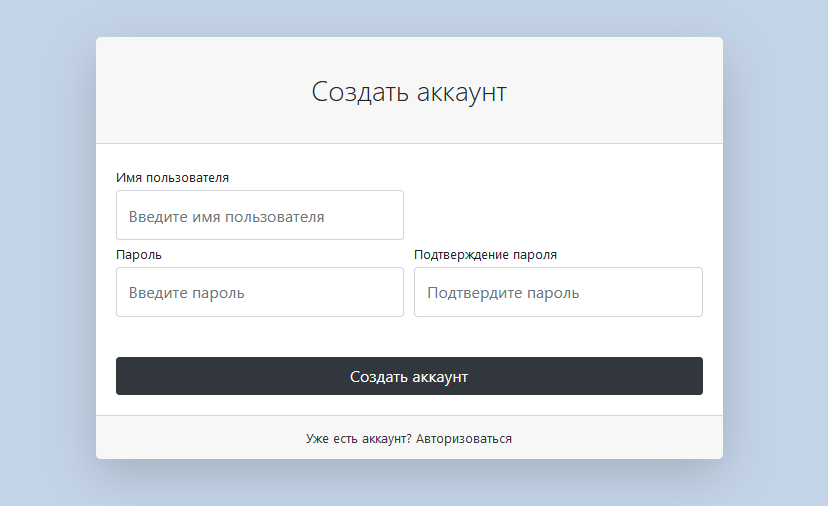
\includegraphics[width=0.8\textwidth]{assets/registration.png} 
        \caption{Страница регистрации}
    \end{figure}
    \begin{figure}[H]
        \centering
        
\includegraphics[width=0.8\textwidth]{assets/index.png} 
        \caption{Главная страница}
    \end{figure}
    \begin{figure}[H]
        \centering
        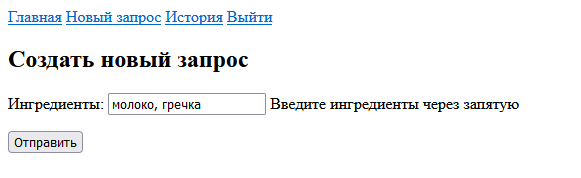
\includegraphics[width=0.8\textwidth]{assets/request.png} 
        \caption{Страница составления запроса}
    \end{figure}
    \begin{figure}[H]
        \centering
        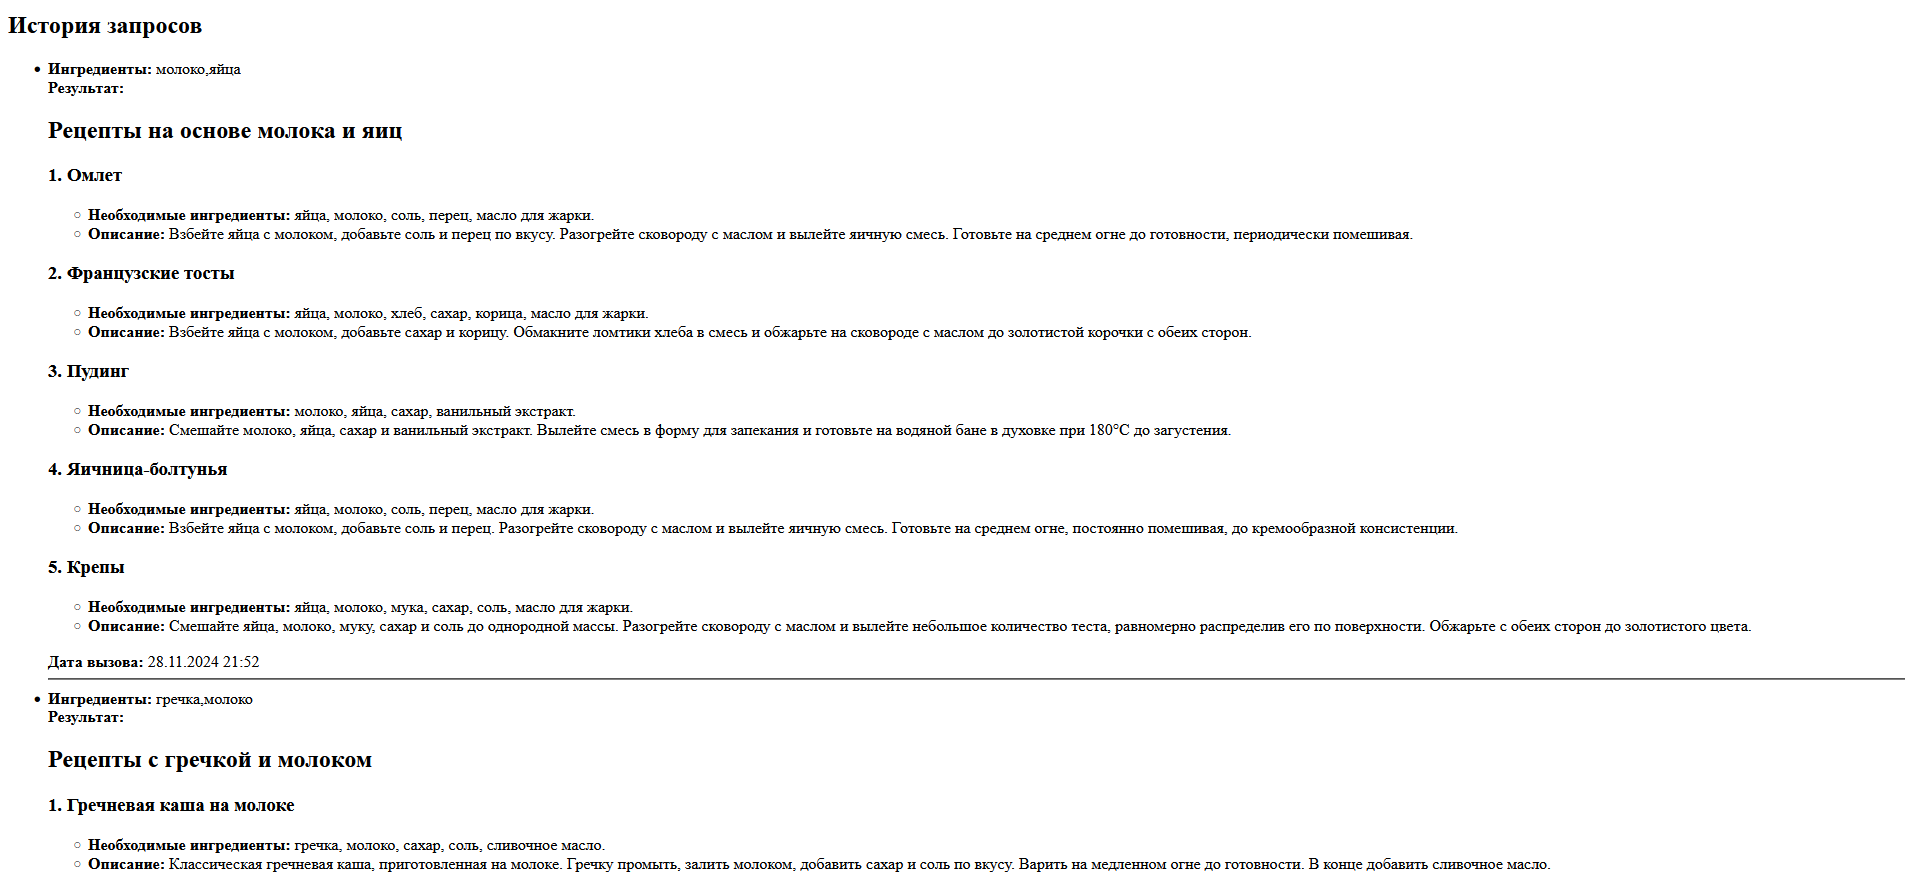
\includegraphics[width=0.8\textwidth]{assets/requests_history.png} 
        \caption{Страница с историей запросов}
    \end{figure}
    
    \subsubsection*{Обработка ошибок и сообщений}
    
    Для улучшения пользовательского опыта были реализованы сообщения об ошибках и успешных действиях. Например, если введен некорректный список ингредиентов или произошла ошибка при запросе рецептов, пользователю выводится соответствующее уведомление. Сообщения об ошибках, такие как недействительный формат ингредиентов, либо серверные ошибки, также отображаются на странице, помогая пользователю быстро выявить и исправить проблему.
    
    \subsubsection*{Технологии и инструменты}
    
    Клиентская часть приложения использует только HTML для создания структуры страницы и CSS для стилизации. Для работы с формами и динамическим отображением данных используется механизм Django шаблонов, который позволяет гибко интегрировать серверную логику с фронтендом. Все элементы формы, такие как поля для ввода и кнопки, обрабатываются с помощью стандартных HTML элементов.
    
    Кроме того, использовались стандартные инструменты Django для обработки данных, их отображения и взаимодействия с сервером, что позволяет эффективно связывать серверную часть и клиентскую часть приложения.
    
}

\newpage

\section{\MakeUppercase{Тестирование приложения}}
Тестирование приложения является важным этапом разработки, так как оно позволяет убедиться в правильности функционирования всех компонентов, выявить возможные ошибки и улучшить пользовательский опыт. В процессе тестирования было проверено несколько ключевых аспектов приложения, таких как корректность работы бизнес-логики, безопасность данных, удобство интерфейса и производительность.

\subsection{Виды тестирования}

В процессе разработки приложения были использованы следующие виды тестирования:

\begin{itemize}
    \item \textbf{юнит-тестирование:} Для проверки отдельных частей кода, таких как функции и методы, использовались юнит-тесты. Юнит-тесты позволяют удостовериться в правильности логики обработки данных, а также в отсутствии ошибок при работе с базой данных и внешними сервисами;
    \item \textbf{интеграционное тестирование:} Интеграционные тесты проверяют взаимодействие различных компонентов приложения, таких как форма запроса ингредиентов, обработка данных на сервере и взаимодействие с внешними сервисами (нейронной сетью). Были протестированы сценарии, связанные с сохранением истории запросов и выводом результатов на клиентскую сторону;
    \item \textbf{тестирование пользовательского интерфейса:} Для проверки удобства и доступности интерфейса были проведены тесты с реальными пользователями. Проверялись различные сценарии использования приложения, такие как регистрация, ввод ингредиентов, получение рецептов и отображение истории запросов;
    \item \textbf{нагрузочное тестирование:} Важно убедиться, что приложение способно эффективно работать при высокой нагрузке, особенно при большом количестве одновременных пользователей. Нагрузочные тесты позволяют оценить производительность системы, выявить узкие места и оптимизировать работу приложения;
    \item \textbf{безопасностное тестирование:} В целях обеспечения безопасности личных данных пользователей и защиты от атак были проведены тесты на уязвимости, такие как SQL-инъекции, XSS-атаки и защита сессий. Проверялись механизмы авторизации и аутентификации, а также безопасность взаимодействия с базой данных.
\end{itemize}

\subsection{Инструменты и методы тестирования}

Для тестирования были использованы следующие инструменты:

\begin{itemize}
    \item \textbf{django Test Framework:} Для юнит-тестирования и интеграционного тестирования использовался встроенный фреймворк Django для тестирования. Он позволяет легко создавать тесты для моделей, представлений и форм, а также предоставляет утилиты для работы с базой данных в тестовом окружении;
    \item \textbf{selenium:} Для тестирования пользовательского интерфейса был использован Selenium — инструмент для автоматизированного тестирования веб-приложений. С его помощью были протестированы взаимодействия пользователя с формами на веб-странице, а также проверено корректное отображение данных на странице;
    \item \textbf{JMeter:} Для нагрузочного тестирования использовался Apache JMeter, который позволяет симулировать большое количество запросов от пользователей и проверять производительность системы при высоких нагрузках;
    \item \textbf{OWASP ZAP:} Для тестирования безопасности использовался инструмент OWASP ZAP (Zed Attack Proxy), который помогает выявить уязвимости в веб-приложении, такие как SQL-инъекции, XSS-уязвимости и другие.
\end{itemize}

\subsection{Результаты тестирования}

\subsubsection*{Юнит-тестирование}
Все юнит-тесты, проверяющие логику работы с базой данных, бизнес-логику и взаимодействие с нейронной сетью, прошли успешно. Все функции, такие как сортировка ингредиентов, проверка существования записей в базе данных и создание новых запросов, работают корректно.

\subsubsection*{Интеграционное тестирование}
Интеграционные тесты показали, что все компоненты приложения (форма запроса, серверная логика и вывод данных) работают правильно в совокупности. Были протестированы сценарии с дублирующимися запросами и корректной обработкой запросов, которые уже были сохранены в базе данных.

\subsubsection*{Тестирование пользовательского интерфейса}
Тестирование интерфейса показало, что страницы приложения интуитивно понятны и удобны для пользователей. Все формы правильно обрабатываются, а результаты запросов корректно отображаются. Были выявлены небольшие улучшения, такие как добавление подсказок и улучшение стилизации для мобильных устройств.

\subsubsection*{Нагрузочное тестирование}
Нагрузочные тесты показали, что приложение может справляться с большими объемами запросов без значительного снижения производительности. Однако при увеличении числа одновременных запросов потребовалась оптимизация некоторых частей кода, таких как работа с базой данных, для улучшения скорости ответа системы.

\subsubsection*{Безопасностное тестирование}
Безопасностное тестирование выявило несколько потенциальных уязвимостей, таких как недостаточная защита от CSRF-атак. Все выявленные проблемы были оперативно исправлены с использованием стандартных механизмов Django для защиты от таких атак.

\subsection{Заключение по тестированию}

Тестирование показало, что приложение функционирует стабильно и соответствует требованиям, предъявляемым к нему в рамках курсового проекта. Все компоненты работают корректно, и приложение безопасно для использования. На основе результатов тестирования были внесены улучшения в работу с базой данных, а также оптимизированы части кода для повышения производительности.

\newpage

\section*{\MakeUppercase{Заключение}}
\addcontentsline{toc}{section}{Заключение}
{
    В рамках работы над курсовым проектом было разработано веб-приложение для поиска кулинарных рецептов с использованием нейронной сети. Приложение предоставляет пользователям возможность вводить список ингредиентов, на основе которых система генерирует рецепты с помощью нейронной сети. Также была реализована система авторизации, которая позволяет сохранять историю запросов для каждого пользователя, обеспечивая удобный доступ к ранее полученным результатам.

    В ходе разработки были использованы современные инструменты и технологии, такие как фреймворк Django для создания бэкенда и работы с базой данных PostgreSQL, а также интеграция с нейронной сетью через API. Для взаимодействия с пользователем был разработан простой и удобный интерфейс на базе HTML-шаблонов Django, что позволило создать интуитивно понятный и доступный пользовательский опыт.
    
    В ходе тестирования приложения были проверены его функциональность, безопасность и производительность. Все ключевые аспекты приложения были протестированы с использованием различных методов тестирования, таких как юнит-тестирование, интеграционное тестирование, нагрузочное тестирование и тестирование безопасности. На основе полученных результатов были внесены необходимые улучшения и оптимизации.
    
    Разработка приложения позволила не только углубить знания в области веб-разработки, но и приобрести практический опыт работы с нейронными сетями, а также улучшить навыки в тестировании программных продуктов. 
    
    В результате работы был достигнут поставленный результат — создание полностью функционирующего веб-приложения, которое может эффективно генерировать рецепты на основе списка ингредиентов и предоставлять пользователю историю запросов. Это приложение может быть использовано как в образовательных целях, так и в коммерческих проектах, связанных с кулинарией.
}
\newpage


\section*{Список использованной литературы}
\addcontentsline{toc}{section}{Список использованной литературы}
    \sloppy
    {
        \begin{enumerate}
           \item Django Software Foundation. Django Documentation [Электронный ресурс]. – Режим доступа: https://www.djangoproject.com/. – Дата доступа: 19.11.2024.
        \item OpenAI. GPT-4: Technical Overview [Электронный ресурс]. – Режим доступа: https://openai.com/research/gpt-4. – Дата доступа: 19.11.2024.
        \item Goodfellow, Ian; Bengio, Yoshua; Courville, Aaron. Deep Learning [Электронный ресурс]. – Режим доступа: https://www.deeplearningbook.org/. – Дата доступа: 19.11.2024.  
        \item Web Application Development with Flask [Электронный ресурс]. – Режим доступа: \url{https://realpython.com/tutorials/flask/}. – Дата доступа: 19.11.2024.  

        \end{enumerate}
    }

}

        \NoBgThispage
        \applicationTitlePage

        \backgroundsetup{
                scale=1,
                color=black,
                opacity=1,
                angle=0,
                position=current page.center,
                vshift=0cm, hshift=0cm,
                contents={
\includegraphics[width=\paperwidth,height=\paperheight]{application/border11.png}}
        }

        \applicationContent
    
\end{document}
